\documentclass[12pt]{article}

\usepackage{pablo-devoir}
\usepackage{pablo-listings}
\usepackage[a5paper,margin=1cm]{geometry}

\pagestyle{empty}

\title{Fonctions}
\date{2/12/14}
\classe{2\up{des}14}
\dsnum{DS 3}

\begin{document}

\maketitle

\begin{exercice}[Images et antécédents --- 7 points]
  \emph{Répondre aux questions par lecture graphique.}
  \begin{enumerate}
    \item On considère la fonction $f$ représentée ci-dessous.
  \begin{center}
    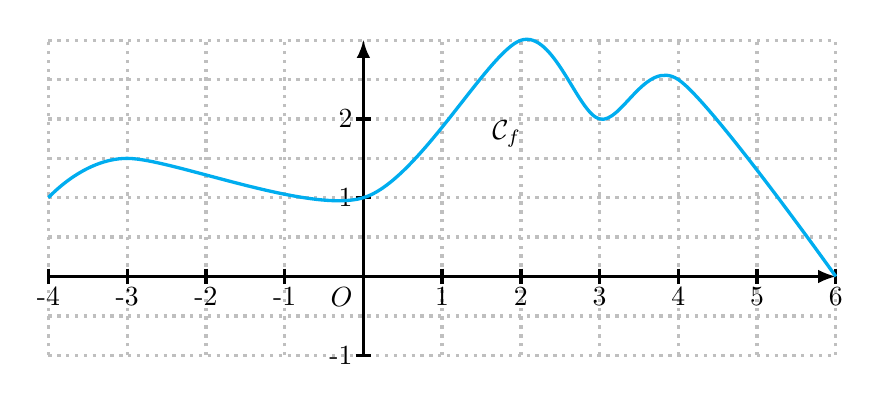
\begin{tikzpicture}[very thick,xscale=1, yscale=1]
      \draw[dotted, lightgray, xstep=1, ystep=.5] (-4, -1) grid (6, 3);
      \draw[-latex] (-4,0) -- (6,0);
      \draw[-latex] (0,-1) -- (0,3);
      \foreach \x in {-4, -3, -2, -1, 1, 2, 3, 4, 5, 6} {
        \draw (\x,0) node[below]{\x};
        \draw (\x,{0.1}) -- (\x,{-0.1});
      }
      \foreach \y in {-1, 1, 2} {
        \draw (0,\y) node[left]{\y};
        \draw (-.1, \y) -- (.1, \y);
      }
      \draw [cyan] plot [smooth, tension=0.5] coordinates {
        (-4,1)
        (-3, 1.5)
        (0, 1)
        (2, 3)
        (3, 2)
        (4, 2.5)
        (6, 0)
      };
      \draw (0,0) node[below left]{$O$};
      \draw (1.5, 1.5) node[above right]{$\mathcal{C}_f$};
    \end{tikzpicture}
  \end{center}
      \begin{enumerate}
        \item Déterminer $f(1)$.
        \item Déterminer l'image de $2$ par $f$.
        \item Quels sont le(s) antécédent(s) de $2$ par $f$ ?
        \item Résoudre graphiquement $f(x)=-1$.
        \item Déterminer un nombre $k$ tel que $f(x)=k$ ait une seule solution.
      \end{enumerate}
    \item Déterminer les solutions de $g(x)=h(x)$ (où les courbes de $g$ et $h$ sont représentées ci-dessous).
      \begin{center}
        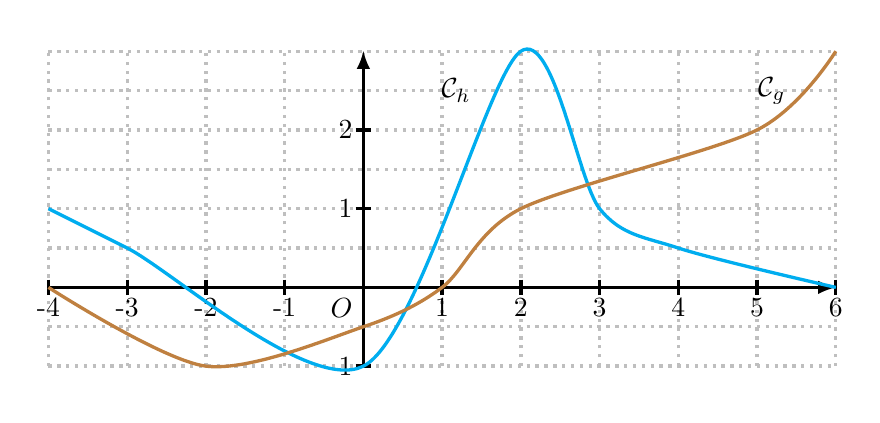
\begin{tikzpicture}[very thick,xscale=1, yscale=1]
          \draw[dotted, lightgray, xstep=1, ystep=.5] (-4, -1) grid (6, 3);
          \draw[-latex] (-4,0) -- (6,0);
          \draw[-latex] (0,-1) -- (0,3);
          \foreach \x in {-4, -3, -2, -1, 1, 2, 3, 4, 5, 6} {
            \draw (\x,0) node[below]{\x};
            \draw (\x,{0.1}) -- (\x,{-0.1});
          }
          \foreach \y in {-1, 1, 2} {
            \draw (0,\y) node[left]{\y};
            \draw (-.1, \y) -- (.1, \y);
          }
          \draw [cyan] plot [smooth, tension=0.5] coordinates {
            (-4,1)
            (-3, 0.5)
            (0, -1)
            (2, 3)
            (3, 1)
            (4, 0.5)
            (6, 0)
          };
          \draw [brown] plot [smooth, tension=0.5] coordinates {
            (-4,0)
            (-2, -1)
            (0, -.5)
            (1, 0)
            (2, 1)
            (5, 2)
            (6, 3)
          };
          \draw (0,0) node[below left]{$O$};
          \draw (1.5, 2.5) node[left]{$\mathcal{C}_h$};
          \draw (5.5, 2.5) node[left]{$\mathcal{C}_g$};
        \end{tikzpicture}
      \end{center}
  \end{enumerate}

\end{exercice}

\begin{exercice}[Variations --- 4 points]
  Voici le tableau de variations d'une fonction $f$.

      \begin{center}
        \begin{tikzpicture}[xscale=1,yscale=1]
          \tkzTabInit[lgt=1,espcl=2]
          {$x$ /1,
            $f$ /2
          }
          {0, 2, 4, 5}%
          \tkzTabVar{-/1, +/2, -/1, +/4}
        \end{tikzpicture}
      \end{center}
      \begin{enumerate}
        \item Comparer $f(3)$ et $f(4)$.
        \item Tracer la courbe d'une fonction $f$ pouvant correspondre à ce tableau.
      \end{enumerate}
\end{exercice}

\begin{exercice}[Algorithme --- 2 points]
  Dans un magasin, le tarif des photocopies est le suivant :
  \begin{itemize}[$\bullet$]
    \item Les vingt premières photocopies : 0,1~\euro{} pièce ;
    \item Les trente suivantes : 0,05~\euro{} pièce ;
    \item Toutes les autres : 0,01~\euro{} pièce.
  \end{itemize}

  Recopier sur votre copie l'algorithme suivant, et le compléter, pour qu'étant donné un nombre $n$, il affiche le prix de $n$ photocopies.
      \begin{lstlisting}[language=naturel,frame=lines,mathescape=true]
      Lire n
      Si ...
      Alors
        Afficher 0,1 * n
      Sinon
        ...
      FinSi
      \end{lstlisting}
\end{exercice}

\begin{exercice}[Problème --- 7 points]
  Une fermière dispose de 100~m de cloture pour faire paître ses moutons. Elle souhaite faire une cloture rectangulaire qui ait la plus grande aire possible.

  \begin{center}
    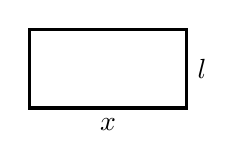
\begin{tikzpicture}[very thick]
      \draw (0,0) -- ++(2, 0) node[midway, below]{$x$} -- ++(0,1) node[midway, right]{$l$} --  ++(-2, 0) -- cycle;
    \end{tikzpicture}
  \end{center}
  On appelle $x$ et $l$ les longueurs des côtés en mètres.
  \begin{enumerate}
    \item 
      \begin{enumerate}
        \item Exprimer le périmètre en fonction de $x$ et $l$.
        \item En déduire que $l=50-x$.
      \end{enumerate}
    \item On appelle $\mathcal{A}(x)$ l'aire de l'enclos, en $m^2$, en fonction de $x$.
      \begin{enumerate}
        \item Quel est le domaine de définition de $\mathcal{A}$ ?
        \item Montrer que $\mathcal{A}(x)=x\left( 50-x \right)$.
      \end{enumerate}
    \item Le tableau de variations de $\mathcal{A}$ est le suivant.
      \begin{center}
        \begin{tikzpicture}[xscale=1,yscale=1]
          \tkzTabInit[lgt=1,espcl=2]
          {$x$ /1,
            $\mathcal{A}$ /2
          }
          {0, 25, 50}%
          \tkzTabVar{-/0, +/625, -/0}
        \end{tikzpicture}
      \end{center}
      Quel est l'aire maximale que peut prendre l'enclos ? Quelle est alors la forme de l'enclos ?
    \item \emph{Bonus} Avec la même longueur de cloture, est-il possible de faire un enclos encore plus grand ?
  \end{enumerate}
\end{exercice}
\end{document}
